\documentclass[../../main/main.tex]{subfiles}
\graphicspath{{./figures/}}

\dominitoc
\faketableofcontents

\makeatletter
\renewcommand{\@chapapp}{\'Electrocin\'etique -- chapitre}
\makeatother

% \toggletrue{student}
% \HideSolutionstrue

\begin{document}
\setcounter{chapter}{3}

\chapter{Oscillateurs harmonique et amorti}

\vfill

\begin{prgm}
	\begin{tcb}*(ror)"know"{Savoirs}
		\begin{itemize}[label=$\diamond$, leftmargin=10pt]
			\item Analyser, sur des relevés expérimentaux, l'évolution de la forme des
			      régimes transitoires en fonction des paramètres caractéristiques.
			\item Prévoir l'évolution du système à partir de considérations
			      énergétiques.
			\item Écrire sous forme canonique l'équation différentielle afin
			      d'identifier la pulsation propre et le facteur de qualité.
			\item Décrire la nature de la réponse en fonction de la valeur du facteur
			      de qualité.
		\end{itemize}
	\end{tcb}

	\begin{tcb}*(ror)"how"{Savoir-faire}
		\begin{itemize}[label=$\diamond$, leftmargin=10pt]
			\item Établir et reconnaître l'équation différentielle qui caractérise un
			      oscillateur harmonique ; la résoudre compte tenu des conditions
			      initiales.
			\item Caractériser l'évolution en utilisant les notions d'amplitude, de
			      phase, de période, de fréquence, de pulsation.
			\item Réaliser un bilan énergétique.
			\item Déterminer la réponse détaillée dans le cas d'un régime libre ou
			      d'un système soumis à un échelon en recherchant les racines du
			      polynôme caractéristique.
			\item Déterminer un ordre de grandeur de la durée du régime transitoire
			      selon la valeur du facteur de qualité.
		\end{itemize}
	\end{tcb}
\end{prgm}

\vfill
\minitoc
\vfill

\newpage

Dans le chapitre précédent, nous avons vu des systèmes qui présentent un régime
transitoire caractérisé par des exponentielles croissantes ou décroissantes. En
combinant deux de ces composants, on trouve alors des régimes transitoires
caractérisé par une combinaison d'exponentielles, exprimée sous la forme de
fonctions sinusoïdales. Regardons un exemple.

\section{Oscillateurs harmoniques}
\subsection{Introduction harmonique}

\subsubsection{Signal sinusoïdal}

\begin{tcbraster}[raster columns=2, raster equal height=rows]
	\begin{tcb}[label=def:signsu](defi){Signal sinusoïdal}
		Un signal sinusoïdal est un signal de la forme
		\psw{
			\[
				\boxed{s(t) = A\cos(\wt + \f)}
			\]
		}
		$A$ est l'\textit{amplitude}, telle que
		\psw{
			\[
				A = \frac{s_{\max} - s_{\min}}{2}
			\]
		}
		$\wt +\f$ est la \textit{phase instantanée} du signal, avec
		\vspace*{-20pt}
		\begin{center}
			\begin{tikzpicture}[]
				\node[anchor=center] (name) at (0,0)
				{\textcolor{cornflowerblue}{$\w$}$t$+\textcolor{limegreen}{$\f$}};
				\node[inner sep=0] (datab) at ([shift={(0,3pt)}]name.south west) {};
				\node[inner sep=0] (biasb) at ([shift={(0,3pt)}]name.south east) {};
				\node[below left =.5cm and .5cm of datab, color=cornflowerblue] (data)
				{pulsation};
				\node[below right=.5cm and .5cm of biasb, color=limegreen] (bias)
				{phase initiale};
				\draw[-stealth] (data) -- (datab);
				\draw[-stealth] (bias) -- (biasb);
			\end{tikzpicture}
		\end{center}
		\tcbsubtitle{\fatbox{Unités}}
		La phase s'exprime en \textbf{radians}~; la pulsation en
		\textbf{$\si{rad.s^{-1}}$}.
	\end{tcb}
	\begin{tcb}[label=exem:graph](exem)'r'{Graphique}
		\begin{center}
			\switch{
				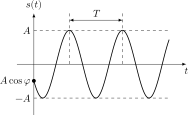
\includegraphics[width=\linewidth, draft=true]{ch8-fig1}
			}{
				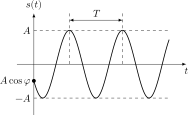
\includegraphics[width=\linewidth]{ch8-fig1}
			}
			\captionof{figure}{}
		\end{center}
		La pulsation représente la \textbf{vitesse avec de variation de la phase}.
		Pour une variation de $2\pi$ effectuée à la période $T$, on définit
		\psw{
			\[
				\boxed{\w = 2 \frac{\pi}{T} = 2\pi f}
				\Lra
				\boxed{T = \frac{2\pi}{\w}}
			\]
		}
		\vspace{-15pt}
	\end{tcb}
\end{tcbraster}

\subsubsection{Équation différentielle oscillateur harmonique}

\begin{tcbraster}[raster columns=2, raster equal height=rows]
	\begin{tcb}[label=prop:eqdiffoh](prop){Équation différentielle}
		Un oscillateur harmonique à un degré de liberté est un système dont
		l'évolution temporelle est décrite par une grandeur $x(t)$ solution
		d'une équation différentielle du type~:
		\psw{
		\[
			\boxed{ \dv[2]{x}{t} + \w_0{}^2x = \w_0{}^2x_{\rm eq}}
		\]
		}
		Avec $x_{\rm eq}$ la position d'équilibre du système et $\w_0$ la
		pulsation \textbf{propre}.
	\end{tcb}
	\begin{tcb}[label=prop:soluoh](prop)'r'{Solutions}
		La forme générale des solutions d'un oscillateur harmonique s'écrit de
		manière équivalente
		\psw{
			\begin{empheq}[box=\fbox]{gather*}
				x(t) = A'\cos(\w_0 t + \f) + x_{\rm eq}\\
				x(t) = A\cos(\w_0 t) + B\sin(\w_0 t) + x_{\rm eq}
			\end{empheq}
		}
		avec $A'$, $\f$, $A$, $B$ des \textit{constantes d'intégration}.
	\end{tcb}
\end{tcbraster}

\subsubsection{Changement de variable~: de général à homogène}
\begin{tcb}[label=demo:chvar](rema)<lfnt>{Changement de variable}
	Au cours du chapitre précédent, nous avons vu la méthode pour résoudre
	des équations différentielles du premier ordre. Nous avons pu remarquer
	que les équations différentielles entre les échelons montants et
	descendants étaient en tout point similaire si ce n'est pour la présence
	ou non d'un second membre, impliquant la recherche d'une solution
	particulière ou non.

	Le changement de variable permet \textbf{d'éviter de
		chercher une solution particulière constante}.
\end{tcb}
\begin{tcb}[label=prop:chvar](prop){Changement de variable}
	Si $x(t)$ est solution de
	\psw{
	\[
		\boxed{ \dv[2]{x}{t} + \w_0{}^2x = \w_0{}^2x_{\rm eq}}
	\]
	}
	alors $y(t) = x(t) - x_{\rm eq}$ est solution de
	\psw{
		\[
			\boxed{ \dv[2]{y}{t} + \w_0{}^2y = 0}
		\]
	}
\end{tcb}
\begin{tcb}(appl)<lfnt>{}
	Résoudre l'équation du circuit RL montant par changement de variable.
	\tcblower
	\psw{
		L'équation différentielle totale s'écrit
		\[
			\boxed{
				\dv{i}{t} + \frac{1}{\tau}i =
				\frac{1}{\tau}\frac{E}{R}
			}
			\Lra
			\dv{i}{t} + \frac{i-\frac{E}{R}}{\tau} = 0
		\]
		On peut donc définir
		\[
			i_h(t) = i(t) - \frac{E}{R} \quad \Ra \quad \dv{i_h}{t} = \dv{i}{t} + 0
		\]
		donc $i_h$ est solution de
		\[
			\dv{i_h}{t} + \frac{i_h}{\tau} = 0
		\]
		de solution générale
		\[
			i_h(t) = A\exr^{-t/\tau}
		\]
		On peut directement chercher l'expression de $A$ par CI~:
		\[
			i_h(0) = \underbracket[1pt]{i(0)}_{=0} - \frac{E}{R} = A
		\]
		Et en ré-isolant $i(t)$, on trouve bien
		\[
			\boxed{i(t) = \frac{E}{R}\left( 1 - \exr^{-t/\tau} \right)}
		\]
	}
	\vspace{-15pt}
\end{tcb}

\subsubsection{Exemple expérimental~: l'oscillateur LC}

Soit le circuit suivant sous un échelon de tension descendant. On observe la
tension $u_C(t)$ avec un oscilloscope dont la courbe est représentée à droite.
\textbf{Une simulation est disponible en
	ligne\ftn{\url{https://tinyurl.com/yl9rvpqg}}}.

\begin{minipage}{0.50\linewidth}
	\begin{center}
		\switch{
			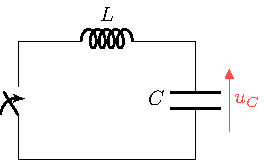
\includegraphics[width=\linewidth, draft=true]{lc_descendant}
		}{
			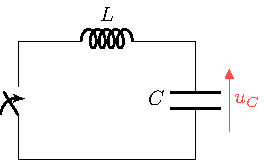
\includegraphics[width=\linewidth]{lc_descendant}
		}
		\captionof{figure}{}
	\end{center}
\end{minipage}
\begin{minipage}{0.50\linewidth}
	\begin{center}
		\switch{
			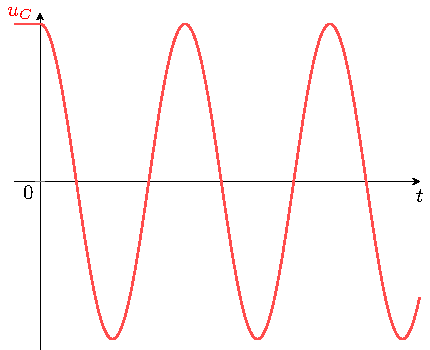
\includegraphics[width=.7\linewidth,
				draft=true]{carac-lc_descendant-harmonique-intro}
		}{
			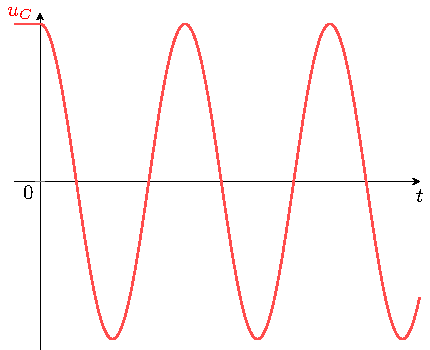
\includegraphics[width=.7\linewidth]{carac-lc_descendant-harmonique-intro}
		}
		\captionof{figure}{}
	\end{center}
\end{minipage}
On remarque que la tension aux bornes du condensateur réalise des
d'oscillations sinusoïdales amorties. En fonction des valeurs des
caractéristiques des composants, on trouve~:
\begin{itemize}
	\item Pour $C_1 = \SI{80}{nF}$ et $L_1 = \SI{43}{mH}$, un période de $T_1 =
		      \SI{364}{\micro s}$~;
	\item Pour $C_2 = \SI{20}{nF}$ et $L_2 = \SI{43}{mH}$, un période de $T_2 =
		      \SI{184}{\micro s}$~;
\end{itemize}

\begin{tcb}(expe){Analyse}
	Lorsque l'on excite le système LC, la tension aux bornes du condensateur
	oscille de façon régulière et sinusoïdale, avec une période qui ne dépend pas
	de l'amplitude de l'excitation mais des caractéristiques de l'oscillateur
	(capacité du condensateur et inductance de la bobine).
\end{tcb}

C'est ce que nous allons maintenant démontrer analytiquement.

\subsection{Oscillateur harmonique électrique~: circuit LC régime
	libre}\label{sec:lclibre}

\subsubsection{Présentation}

\begin{minipage}[c]{.6\linewidth}
	\begin{itemize}
		\item Il est constitué de l'association en série d'une bobine et d'un
		      condensateur idéaux.
		\item \textbf{On suppose le condensateur initialement chargé}~:
		      \fbox{$u_C(0^-) = E$ \underline{et} $i(0^-) = 0$} (condensateur chargé
		      $\equiv$ interrupteur ouvert).
		\item À $t=0$, on coupe le générateur.
	\end{itemize}
\end{minipage}
\hfill
\begin{minipage}[c]{.35\linewidth}
	~
	\begin{center}
		\switch{
			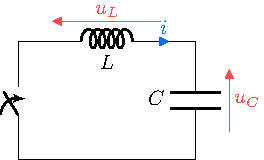
\includegraphics[width=.9\linewidth, draft=true]{lc_descendant-intens}
		}{
			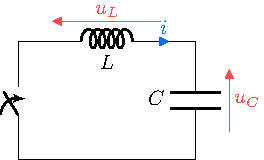
\includegraphics[width=.9\linewidth]{lc_descendant-intens}
		}
		\captionof{figure}{}
	\end{center}
\end{minipage}

\subsubsection{Équation différentielle du circuit}
\begin{tcb}[label=demo:eqdiffrc](demo)<lfnt>{Équation diff. LC libre}
	Avec la loi des mailles,
	\psw{
		\begin{DispWithArrows*}[]
			u_L + u_C &= 0
			\Arrow{$\DS u_L = L \dv{i}{t}$\\ et $\DS i = C \dv{u_C}{t}$}
			\\\Lra
			LC \dv[2]{u_C}{t} + u_C          &= 0
			\Arrow{forme canonique}
			\\
			\Lra \dv[2]{u_C}{t} + \frac{1}{LC}u_C &= 0
		\end{DispWithArrows*}
		D'où le résultat. $L$ assure $i(0^+) = 0$ et $C$ assure $u_C(0^+) = E$
		par continuité.
	}
\end{tcb}
\begin{tcb}[label=prop:eqdiffrc, sidebyside, righthand ratio=.4](prop){Équation diff. LC libre}
	L'équation différentielle de la tension $u_C(t)$ aux bornes d'un
	condensateur dans un circuit LC en régime libre est
	\psw{
		\[
			\boxed{\dv[2]{u_C}{t} + \w_0{}^2u_C = 0}
		\]
	}
	avec \fbox{$\w_0 = \frac{1}{\sqrt{LC}}$} la pulsation propre.
	\tcblower
	Les conditions initiales (continuité de $u_C$ aux bornes de $C$
	et de $i$ traversant $L$) sont
	\psw{
		\begin{empheq}[box=\fbox]{gather*}
			u_C(0^-) = u_C(0^+) = E\\
			i(0^-) = i(0^+) = 0
		\end{empheq}
	}
\end{tcb}

\begin{tcb}[label=rema:unité](appl){Unité de $\w_0$}
	On peut vérifier à cette étape que $\w_0$ est bien homogène à l'inverse d'un
	temps. Pour ça, deux manières~:

	\begin{isd}[sidebyside align=top]
		\tcbsubtitle{\fatbox{Analyse directe}}
		Sachant que $RC$ et $L/R$ sont des temps (cf.\ chapitre précédent)~:
		\psw{
			\begin{align*}
				w_0{}^2 = \frac{1}{LC} =
				\frac{R}{LRC} =
				\underbrace{\left[ \frac{L}{R}
						\right]^{-1}}_{\si{s^{-1}}}\times
				\underbrace{\left[ RC \right]^{-1}}_{\si{s^{-1}}}
			\end{align*}
			Et on a bien $\w_0{}^2$ en \si{s^{-2}}, et donc $\w_0$ en \si{s^{-1}},
			les radians n'ayant pas de dimension.
		}
		\tcblower
		\tcbsubtitle{\fatbox{Analyse indirecte}}
		En effet, l'équation différentielle est forcément une équation homogène.
		Ainsi
		\psw{
			\begin{equation*}
				\left[ \dv[2]{u_C}{t} \right] =
				\frac{\left[u_C\right]}{\left[\dt\right]^2}\\
				= \frac{\si{V}}{\si{s^2}}
			\end{equation*}
			et l'autre terme doit avoir la même unité~:
			\begin{equation*}
				\left[ w_0{}^2u_C \right] = \left[ w_0 \right]^2\times \left[
					u_C \right]\\
				= \si{V.s^{-2}}
			\end{equation*}
			On en déduit que $\w_0{}^2$ est de dimension \si{s^{-2}}, d'où la
			dimension de $\w_0$.
		}
	\end{isd}
\end{tcb}

\subsubsection{Résolution de l'équation différentielle et graphique}
\begin{tcb}[label=demo:rcsolu](demo)<lfnt>{Solutions LC série descendant}
	L'équation étant déjà homogène, on écrit la forme générale~:
	\psw{
		\[
			u_C(t) = A\cos(\w_0 t) + B\sin(\w_0 t)
		\]
	}
	\vspace{-15pt}
	\begin{itemize}
		\item On trouve $A$ avec la première condition initiale~:
		      \psw{
			      \[
				      u_C(0) = A\cos(0) + B\sin(0) = A
				      \qet
				      u_C(0) = E
				      \quad \Ra \boxed{A = E}
			      \]
		      }
		      \vspace{-15pt}
		\item On trouve $B$ avec la seconde condition initiale~:
		      \psw{
			      \begin{gather*}
				      \dv{u_C}{t} = -A\w_0\sin(\w_0t) + B\w_0\cos(\w_0t)
				      \Ra \dv{u_C}{t}\/(0) = B\w_0
				      \\
				      \text{et} \quad
				      i(0) = 0 = C \dv{u_C}{t}\/(0) = CB\w_0
				      \quad \Ra \boxed{B = 0}
			      \end{gather*}
		      }
		      \vspace{-15pt}
	\end{itemize}
	On obtient ensuite $i$ avec la relation courant-tension~:
	\psw{
		\[
			i(t) = C \dv{u_c}{t} = -CE \w_0 \sin(\w_0t)
		\]
	}
	\vspace{-15pt}
\end{tcb}
\begin{tcbraster}[raster columns=2, raster equal height=rows]
	\begin{tcb}[label=prop:ucsolu](prop){Solution de l'équation
				différentielle LC}
		La solution de l'équation différentielle de la tension $u_C(t)$
		d'un circuit LC en décharge avec $u_C(0) = E$ et l'intensité en
		découlant sont
		\psw{
			\begin{empheq}[box=\fbox]{gather*}
				u_C(t) = E\cos(\w_0t)\\
				i(t) = -CE\w_0\sin(\w_0t)
			\end{empheq}
		}
	\end{tcb}
	\begin{tcb}[width=\linewidth](exem)'r'{Graphique}
		\begin{center}
			\switch{
				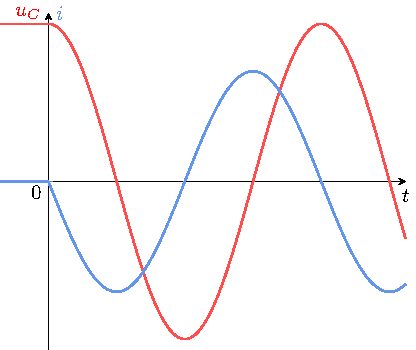
\includegraphics[width=\linewidth,
					draft=true]{carac-lc_descendant-harmonique}
			}{
				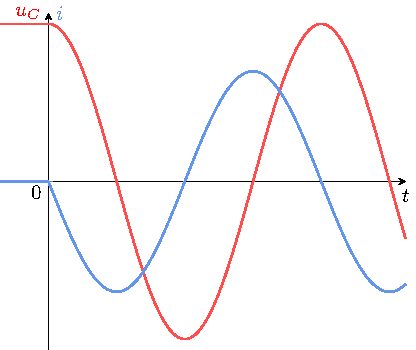
\includegraphics[width=\linewidth]{carac-lc_descendant-harmonique}
			}
			\captionof{figure}{}
		\end{center}
	\end{tcb}
\end{tcbraster}

\subsubsection{Bilan énergétique}
\begin{tcb}[label=demo:rcenerg-charge](demo)<lfnt>{Bilan d'énergie}
	On fait un bilan de puissances avec la loi des mailles multipliée par $i$~:
	\psw{
		\begin{DispWithArrows*}
			u_Ci + u_Li &= 0
			\Arrow{$i = C \dv{u_C}{t}$\\et $u_L = L \dv{i}{t}$}
			\\
			\Lra
			u_C\times C \dv{u_C}{t} + L \dv{i}{t}\times i &= 0
			\Arrow{$f \times f' = \left( \frac{1}{2}f^{2} \right)'$}
			\\\Lra
			\dv{}{t} \left( \frac{1}{2}Cu_C{}^2 + \frac{1}{2}Li^2 \right) &= 0
		\end{DispWithArrows*}
		On identifie l'intérieur de la parenthèse à l'énergie du système (car
		par définition $\Pc = \dv{\Ec}{t}$) pour avoir la propriété.
	}
\end{tcb}
\begin{tcbraster}[raster columns=2, raster equal height=rows]
	\begin{tcb}[label=prop:lcenerg-décharge](prop){Bilan d'énergie}
		L'énergie emmagasinée dans le circuit est
		\psw{
		\[
			\boxed{\Ec = \frac{1}{2}Cu_C{}^2 + \frac{1}{2}Li^2}
		\]
		}
		Elle est \textbf{conservée à chaque instant} et résulte de l'\textbf{échange
			périodique} d'énergie entre le condensateur et la bobine.
	\end{tcb}
	\begin{tcb}[width=\linewidth](exem)'r'{Graphique}
		\begin{center}
			\switch{
				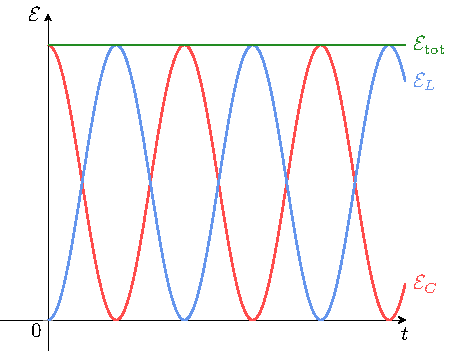
\includegraphics[width=\linewidth, draft=true]{carac-lc_descendant-bilan}
			}{
				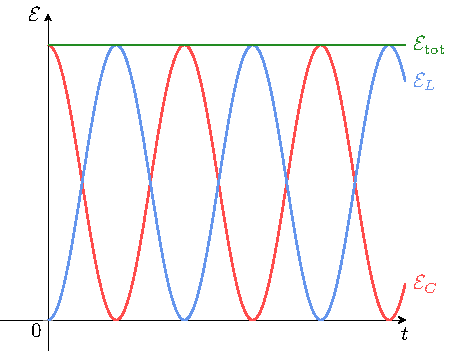
\includegraphics[width=\linewidth]{carac-lc_descendant-bilan}
			}
			\captionof{figure}{}
		\end{center}
	\end{tcb}
\end{tcbraster}

\begin{tcb}[label=impl](impl){Vérification conservation de l'énergie}
	On vérifie avec les expressions analytiques trouvées, sachant que
	$\w_0{}^2 = (LC)^{-1}$~:
	\psw{
		\begin{align*}
			\frac{1}{2}Cu_C{}^2 & = \frac{1}{2}CE^2\cos^2(\w_0t)
			\\
			\text{et} \quad
			\frac{1}{2}Li^2     & =
			\frac{1}{2}\underbracket[1pt]{LC^{2}\w_0{}^2}_{=C}E^2\sin^2(\w_0t)
			\\\Ra
			\Ec                 & = \frac{1}{2}CE^2 \left( \cos^2(\w_0t) + \sin^2(\w_0t) \right)
		\end{align*}
		Soit
		\begin{equation*}
			\boxed{\Ec = \frac{1}{2}CE^2 = \text{cste}}
		\end{equation*}
	}
\end{tcb}
\begin{tcb}[label=impo:amortissement](impo){Résultat}
	On retrouve bien des oscillations de la tension aux bornes de $u_C$ comme dans
	l'approche expérimentale, avec une période $T_0 = \frac{2\pi}{\w_0} =
		2\pi\sqrt{LC}$ qui augmente avec $L$ et $C$.
	\bigbreak
	Il n'y a donc \textbf{pas d'amortissement ici}~! En effet les composants
	utilisés ici sont idéaux, et conservent totalement l'énergie, il n'y a pas de
	raison d'en perdre.
	\bigbreak
	Il y a eu une simplification que l'on effectue souvent en mécanique~:
	\textbf{on a négligé les effets dissipatifs}. Regardons comment ça se traduit
	pour un exemple mécanique.
\end{tcb}

\subsection{Exemple harmonique mécanique~: ressort horizontal libre}

\subsubsection{Introduction}

\begin{tcb}[label=defi:ressortdef, sidebyside, righthand ratio=.5](defi){Force de
			rappel d'un ressort}
	Soit le système masse-ressort horizontal représenté ci-contre. Le ressort se
	déforme sous l'effet d'une contrainte en stockant l'énergie donnée, qu'il
	libère en reprenant sa forme quand la contrainte s'arrête. On définit la
	force de rappel du ressort par~:
	\psw{
		\begin{equation*}
			\boxed{\vv*{F}{\rm rappel} = -k(\ell - \ell_0)\ux}
		\end{equation*}
	}
	\vspace{-15pt}
	\begin{itemize}
		\item $k > 0$ la \textbf{constante de raideur}~;
		\item $\ell_0$ sa \textbf{longueur à vide}~;
		\item $\ux$ un vecteur unitaire \ftn{$ \left\Vert \ux \right\Vert = 1$}
		      dirigé selon $x$.
	\end{itemize}
	\tcbsubtitle{\fatbox{Unité}}
	\psw{
	$k$ en $\si{N.m^{-1}}$ ($[\vv{F}] = [k][\ell]$)
	}
	\tcblower
	\begin{center}
		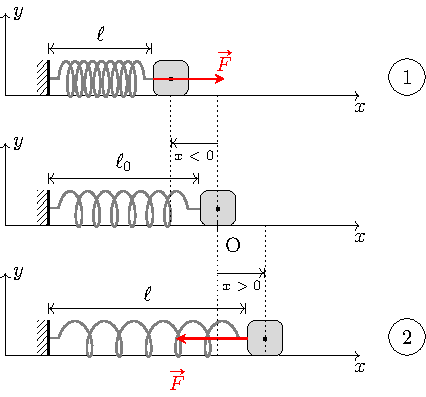
\includegraphics[width=\linewidth]{ressort_def}
		\captionof{figure}{}
	\end{center}
	Si $\ell > \ell_0$, on a bien une force dirigée selon $-\ux$, (situation
	\circled{2}), sinon dirigée selon $+\ux$.
\end{tcb}

\subsubsection{Présentation}
\begin{tcb}[label=def:ressortlibre, sidebyside](defi){Situation
			initiale et bilan des forces}
	\begin{itemize}[label=$\diamond$, leftmargin=10pt]
		\bitem{Système~:} \{point M\} de masse $m$, accroché à un \textbf{ressort
			idéal sans frottements}
		\bitem{Référentiel~:} $\Rc\ind{sol}(O',x,y,t)$ supposé galiléen
		\bitem{Repère~:} $(\Or', \ux, \uy)$ (voir schéma)
		\bitem{Repérage~:}
		\vspace{-15pt}
		\begin{center}
			\hspace*{-10pt}
			\fbox{Soit $x (t) = \ell(t) - \ell_0$ la position de la masse}
		\end{center}
		\[
			\vv{\rm O'M} = x(t)\ux~; \vf = \xp(t)\ux~; \af = \xpp(t)\ux.
		\]
		\bitem{Position initiale~:} ${\rm O'M}(0) = x_0 >0$
		\bitem{Vitesse initiale~:} $\vf(0) = \of$
	\end{itemize}
	\tcblower
	\begin{center}
		\switch{
			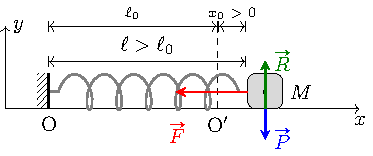
\includegraphics[width=\linewidth, draft=true]{ressort_libre}
		}{
			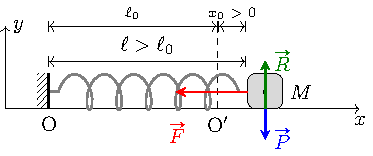
\includegraphics[width=\linewidth]{ressort_libre}
		}
		\captionof{figure}{}
	\end{center}
	\begin{itemize}[label=$\diamond$, leftmargin=10pt]
		\bitem{Bilan des forces~:}
		\psw{
			\[
				\begin{array}{ll}
					\textbf{Poids}            & \Pf = m\gf = -mg \uy \\
					\textbf{Réaction normale} & \Rf = R\uy           \\
					\textbf{Force de rappel}  & \Ff = -kx (t)\ux
				\end{array}
			\]
		}
	\end{itemize}
\end{tcb}

\subsubsection{Équation différentielle et solution}

\begin{tcb}[label=demo:solreslibre, sidebyside, sidebyside align=top](demo)<lfnt>{Équation différentielle et solution}
	\tcbsubtitle{\fatbox{Équation}}
	La deuxième loi de \textsc{Newton}, ou \textbf{principe fondamental de la
		dynamique} (PFD) donne~:
	\psw{
		\begin{gather*}
			\dv{\pf}{t} = m\af = \Pf + \vv{R} + \Ff\\
			\Lra m
			\mqty(
			\dv[2]{x}{t} \\
			0
			)
			=
			\mqty(
			-kx \\
			-mg + R
			)
		\end{gather*}
	}
	Sur l'axe $\ux$\ftn{La projection sur $\uy$ montre que la réaction du support
		compense le poids.} on trouve alors
	\psw{
		\[
			m \dv[2]{x}{t} + kx = 0 \Lra \boxed{\dv[2]{x}{t} + \w_0{}^{2}x = 0}
		\]
	}
	avec
	\psw{
		\[
			\w_0{}^{2} = \frac{k}{m} \Ra \boxed{\w_0 = \sqrt{\frac{k}{m}}}
		\]
	}
	\tcblower
	\tcbsubtitle{\fatbox{Solution}}
	On écrit la forme générale~:
	\psw{
		\[
			x(t) = A\cos(\w_0 t) + B\sin(\w_0 t)
		\]
	}
	\vspace{-20pt}
	\begin{itemize}
		\item On trouve $A$~:
		      \psw{
			      \[
				      x(0) = A
				      \qet
				      x(0) = x_0
				      \quad \Ra \boxed{A = x_0}
			      \]
		      }
		      \vspace{-15pt}
		\item On trouve $B$~:
		      \psw{
			      \begin{gather*}
				      v(0) = 0 = \dv{x}{t}\/(0) = B\w_0
				      \quad \Ra \boxed{B = 0}
			      \end{gather*}
		      }
		      \vspace{-15pt}
	\end{itemize}
	Donc
	\psw{
		\[
			\boxed{x (t) = x_0\cos(\w_0t)}
		\]
	}
	On obtient ensuite $v$ avec la relation vitesse-position.
\end{tcb}
\begin{tcb}[label=prop:eqdiffreslibre, sidebyside, righthand ratio=.4](prop){Équation et solution}
	La position $x$ de la masse et la longueur $\ell$ du ressort sont régies
	par~:
	\psw{
		\begin{empheq}[box=\fbox]{gather*}
			\dv[2]{x}{t} + \w_0{}^2x = 0
			\Lra \dv[2]{\ell}{t} + \w_0{}^2\ell = \w_0{}^2\ell_0
		\end{empheq}
	}
	Avec $\w_0 = \sqrt{\frac{k}{m}}$.
	\smallbreak
	$\ell_0$ est donc la \textbf{longueur d'équilibre} du système.
	\tcblower
	La position $x$ et la vitesse $v$ ont pour expressions
	\psw{
		\begin{empheq}[box=\fbox]{align*}
			x(t) &= x_0\cos(\w_0t)\\
			\text{et} \quad
			v(t) &= -x_0\w_0\sin(\w_0t)
		\end{empheq}
	}
\end{tcb}
\begin{tcb}[label=impo:ressortlibre](impo){Analogie LC-ressort}
	Alors qu'on partait d'un système \textit{a priori} totalement différent, on
	remarque que la physique des deux systèmes sont rigoureusement équivalentes
	puisque \textbf{régies par la même équation différentielle}.
	\bigbreak
	\noindent
	\begin{minipage}[c]{.6\linewidth}
		On observe une oscillation du ressort autour d'une position d'équilibre, ici
		$x=0 \Lra \ell = \ell_0$, tout comme $u_C$ oscille autour de 0.
		\smallbreak
		On associe donc $q$ à $x$ et $i$ à $v$, étant donné que pour un
		condensateur $i = \dv{q}{t}$ et que $v = \dv{x}{t}$.
		\smallbreak
		De plus c'est la \textbf{masse} qui impose l'inertie du mouvement, comme
		l'\textbf{inductance} est l'inertie de l'intensité.
		\smallbreak
		Finalement, $\w_0 = 1/\sqrt{LC}$ en électrocinétique et $\w_0 =
    \sqrt{k/m}$ en mécanique, donc on associe $k$ à $C^{-1}$.
	\end{minipage}
	\begin{minipage}[c]{.39\linewidth}
		\captionof{table}{Correspondances}
		\centering
		\begin{tabular}{c@{$\longleftrightarrow$}c}
			\toprule
			Méca                       & Élec
			\\
			\midrule
			\psw{$x$}                  & \psw{$q$}
			\\
			\psw{$v$}                  & \psw{$i$}
			\\
			\psw{$m$}                  & \psw{$L$}
			\\
			\psw{$k$}                  & \psw{$C^{-1}$}
			\\
			\psw{$\sqrt{\frac{k}{m}}$} & \psw{$\frac{1}{\sqrt{LC}}$}
			\\
			\bottomrule
		\end{tabular}
	\end{minipage}
\end{tcb}

\subsubsection{Bilan énergétique}

\begin{tcb}[label=def:emeca, sidebyside](defi){Énergies potentielle élastique et mécanique}
	Le ressort emmagasine une énergie \textit{potentielle} lors de sa
	déformation, telle que
	\psw{
		\[
			\boxed{
				\Ec_{p\rm, el} = \frac{1}{2}k(\ell-\ell_0)^2 = \frac{1}{2}kx^2
			}
		\]
	}
	\tcblower
	On définit alors l'énergie mécanique totale $\Ec_m$ du système par
	\psw{
		\[
			\boxed{\Ec_m = \Ec_c + \Ec_{p\rm, el}}
		\]
	}
	avec, évidemment, $\Ec_c = \frac{1}{2}mv^2$.
\end{tcb}
\begin{tcb}[fontupper=\Large, bld, cnt](ror){Bilan de puissance en méca}
	On effectue un bilan de puissance en écrivant le PFD multiplié par $v$~:
	$\Pc(\vv{F}) = \vv{F}\cdot \vv{v}$.
\end{tcb}
\begin{tcb}[label=demo:emecacons](demo)<lfnt>{Conservation énergie}
	À partir du PFD~:
	\vspace{-15pt}
	\psw{
		\begin{DispWithArrows*}[]
			m \dv[2]{x}{t} + kx &= 0
			\CArrow{$\times v$}
			\\\Lra
			m \dv[2]{x}{t} \dv{x}{t} + kx \dv{x}{t} &= 0
			\Arrow{$f \times f' = \left(\frac{1}{2}f^2\right)'$}
			\\\Lra
			\dv{}{t}
			\Big(
			\underbracket{\frac{1}{2}m \left( \dv{x}{t} \right)^2}_{\Ec_c} +
			\underbracket{\frac{1}{2}kx^2}_{\Ec_{p, \rm el}}
			\Big) &= 0
		\end{DispWithArrows*}
	}
	\vspace{-15pt}
\end{tcb}
\begin{tcbraster}[raster columns=2, raster equal height=rows]
	\begin{tcb}[label=prop:emecacons](prop){Conservation énergie}
		Dans le système masse-ressort horizontal sans frottements, l'énergie
		mécanique est conservée~:
		\psw{
			\[
				\boxed{\Ec_m = \cte}
				\Lra
				\boxed{\dv{\Ec_m}{t} = 0}
			\]
		}
		\vspace{-15pt}
	\end{tcb}
	\begin{tcb}[width=\linewidth](exem)'r'{Graphique}
		\begin{center}
			\switch{
				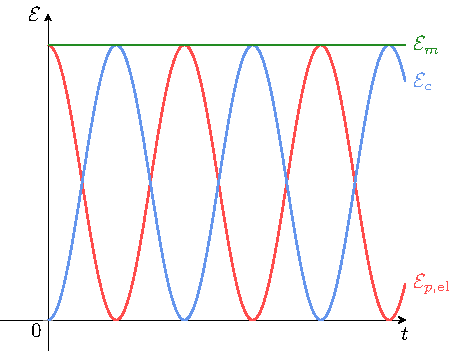
\includegraphics[width=\linewidth,
					draft=true]{carac-ressort_libre-bilan}
			}{
				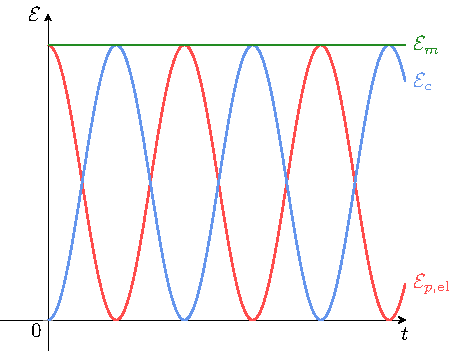
\includegraphics[width=\linewidth]{carac-ressort_libre-bilan}
			}
			\captionof{figure}{}
		\end{center}
	\end{tcb}
\end{tcbraster}
\begin{tcb}[label=impl](impl){Vérification}
	On vérifie avec les expressions analytiques, sachant que
	$\w_0{}^2 = \frac{k}{m}$~:
	\psw{
		\begin{align*}
			\frac{1}{2}kx^2 & = \frac{1}{2}kx_0{}^2\cos^2(\w_0t)
			\\
			\text{et} \quad
			\frac{1}{2}mv^2 & =
			\frac{1}{2}\underbracket[1pt]{m\w_0{}^2}_{=k}x_0{}^2\sin^2(\w_0t)
			\\\Ra
			\Ec_m           & = \frac{1}{2}kx_0{}^2 \left( \cos^2(\w_0t) + \sin^2(\w_0t) \right)
		\end{align*}
		Soit
		\begin{equation*}
			\boxed{\Ec_m = \frac{1}{2}kx_0{}^2 = \text{cste}}
		\end{equation*}
	}
\end{tcb}

\subsubsection{Analyse correspondance}
\begin{tcb}[width=\linewidth, sidebyside, righthand ratio=.4](rema){Espace des
			phases}
	Il est utile d'observer la physique des systèmes oscillants non pas dans
	un espace (grandeur, temps) mais dans un espace \textbf{(grandeur,
		dérivée)}, qui permet plus rapidement de sonder son évolution~: c'est ce
	qu'on appelle \textbf{l'espace des phases}.
	\bigbreak
	Par
	exemple, le ressort lâché à $x_0$ et $v_0=0$ voit sa position diminuer
	et sa vitesse augmenter (algébriquement) jusqu'à ce qu'il passe par sa
	position d'équilibre ($x=0$) avec une vitesse extrémale $v_{\min}$,
	avant de se comprimer en perdant de sa vitesse.
	\bigbreak
	Comme il n'y a
	\textbf{pas de perte dans cette étape}, elle se répète
	\textbf{symétriquement} en revenant à son point de départ.
	\tcblower
	\begin{center}
		\switch{
			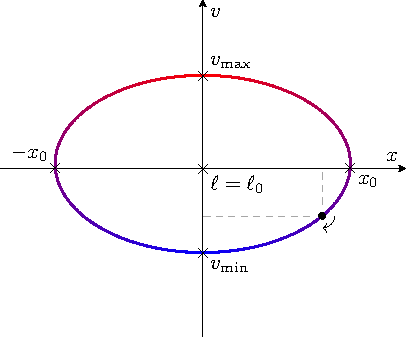
\includegraphics[width=\linewidth, draft=true]{carac-ressort_libre-xy}
		}{
			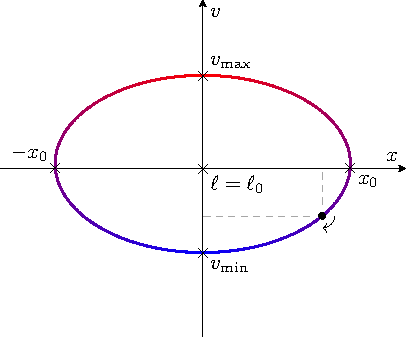
\includegraphics[width=\linewidth]{carac-ressort_libre-xy}
		}
		\captionof{figure}{}
	\end{center}
\end{tcb}

\begin{tcb}[label=impo:harmotoamorti](impo){Conclusion}
	En réalité, les \textbf{frottements en mécanique existent}, et à chaque étape
	le système masse-ressort perd de l'énergie dans la dissipation par frottement
	créant de la chaleur. On va donc avoir une \textbf{trajectoire amortie} plus
	ou moins fortement.
	\bigbreak
	Dans le cas électrique, c'est la \textbf{résistance que nous avions négligée}
	alors qu'elle existe toujours~: notamment la bobine réelle est composée d'une
	bobine idéale et d'une résistance en série. C'est la résistance qui va
	\textbf{dissiper l'énergie} de l'oscillateur harmonique LC sous forme de
	chaleur par effet \textsc{Joule} et amortir l'oscillation de $u_C$.
\end{tcb}

\subsection{Complément~: circuit LC montant}

\subsubsection{Présentation}
\begin{minipage}[c]{.6\linewidth}
	\begin{itemize}
		\item Il est constitué de l'association en série d'un générateur idéal de
          f.e.m. $E$, d'une bobine et d'un condensateur idéaux.
		\item \textbf{On suppose le condensateur initialement déchargé}~:
		      \fbox{$u_C(0^-) = 0$ \underline{et} $i(0^-) = 0$} (condensateur chargé
		      $\equiv$ interrupteur ouvert).
		\item À $t=0$, on allume le générateur\ftn{\url{https://tinyurl.com/ypagwnb6}}.
	\end{itemize}
\end{minipage}
\hfill
\begin{minipage}[c]{.35\linewidth}
	~
	\begin{center}
		\switch{
			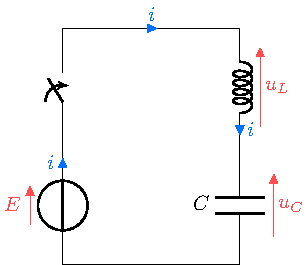
\includegraphics[width=.9\linewidth, draft=true]{lc_montant}
		}{
			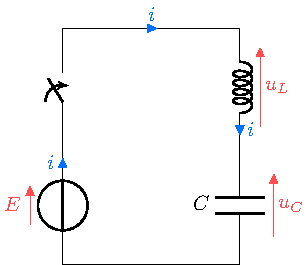
\includegraphics[width=.9\linewidth]{lc_montant}
		}
		\captionof{figure}{}
	\end{center}
\end{minipage}

\subsubsection{Équation différentielle du circuit}
\begin{tcbraster}[raster columns=2, raster equal height=rows]
	\begin{tcb}[label=prop:eqdiffrc](prop){Équation diff. LC montant}
		L'équation différentielle de la tension $u_C(t)$ aux bornes d'un
		condensateur dans un circuit LC sous échelon montant est
		\psw{
			\[
				\boxed{\dv[2]{u_C}{t} + \w_0{}^2u_C = \w_0{}^{2}E}
			\]
		}
		avec \fbox{$\w_0 = \frac{1}{\sqrt{LC}}$} la pulsation propre.
		\tcblower
		Les conditions initiales (continuité de $u_C$ aux bornes de $C$
		et de $i$ traversant $L$) sont
		\psw{
			\begin{empheq}[box=\fbox]{gather*}
				u_C(0^-) = u_C(0^+) = 0\\
				i(0^-) = i(0^+) = 0
			\end{empheq}
		}
	\end{tcb}
	\begin{tcb}[label=demo:eqdiffrc](demo)'r'{Équation diff. LC montant}
		Avec la loi des mailles,
		\psw{
			\begin{DispWithArrows*}[fleqn, mathindent=5pt]
				u_L + u_C &= E
				\Arrow{$\DS u_L = L \dv{i}{t}$\\ et $\DS i = C \dv{u_C}{t}$}
				\\\Lra
				LC \dv[2]{u_C}{t} + u_C          &= E
				\Arrow{forme canonique}
				\\
				\Lra \dv[2]{u_C}{t} + \frac{1}{LC}u_C &= \frac{1}{LC}E
			\end{DispWithArrows*}
			D'où le résultat. $L$ assure $i(0^+) = 0$ et $C$ assure $u_C(0^+) = 0$
			par continuité.
		}
	\end{tcb}
\end{tcbraster}

\subsubsection{Résolution de l'équation différentielle et graphique}
\begin{tcbraster}[raster columns=2, raster equal height=rows]
	\begin{tcolorbox}[blankest, raster multicolumn=1, space to=\myspace]
		\begin{tcbraster}[raster columns=1]
			\begin{tcb}[label=prop:ucsolu](prop){Solution LC montant}
				La solution de l'équation différentielle de la tension $u_C(t)$
				d'un circuit LC en charge avec $u_C(0) = 0$ et l'intensité en
				découlant sont
				\psw{
					\begin{empheq}[box=\fbox]{gather*}
						u_C(t) = E(1 - \cos(\w_0t))\\
						i(t) = CE\w_0\sin(\w_0t)
					\end{empheq}
				}
			\end{tcb}
			\begin{tcb}[width=\linewidth](exem){Graphique}
				\begin{center}
					\switch{
						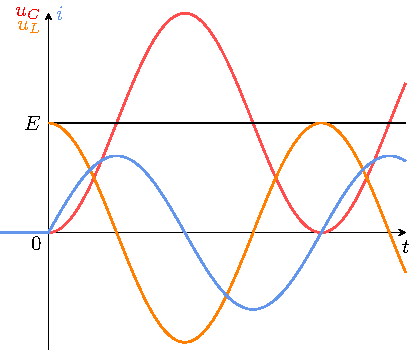
\includegraphics[width=\linewidth,
							draft=true]{carac-lc_montant-harmonique}
					}{
						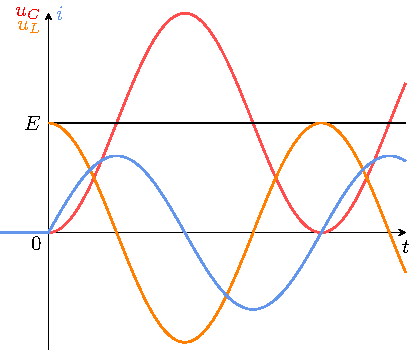
\includegraphics[width=\linewidth]{carac-lc_montant-harmonique}
					}
					\captionof{figure}{}
				\end{center}
			\end{tcb}
		\end{tcbraster}
	\end{tcolorbox}
	\begin{tcb}[label=demo:rcsolu](demo)'r'{Solution LC montant}
		D'après la propriété \ref{prop:chvar}, on sait que $u_C - E$ est
		solution de l'équation homogène associée, donc on a
		\psw{
			\[
				u_C(t) - E = A\cos(\w_0 t) + B\sin(\w_0 t)
			\]
		}
		\vspace{-15pt}
		\begin{itemize}
			\item On trouve $A$~:
			      \psw{
				      \[
					      u_C(0) - E = A
					      \Ra \boxed{A = -E}
				      \]
			      }
			      \vspace{-15pt}
			\item On trouve $B$~:
			      \psw{
				      \begin{gather*}
					      i(0) = 0 = C \dv{u_C}{t}\/(0) = CB\w_0
					      \quad \Ra \boxed{B = 0}
				      \end{gather*}
			      }
			      \vspace{-15pt}
		\end{itemize}
		Donc
		\psw{
			\[
				\boxed{u_C (t) = E \left( 1 - \cos(\w_0t) \right)}
			\]
		}
		On obtient ensuite $i$ avec la relation courant-tension~:
		\psw{
			\[
				i(t) = C \dv{u_c}{t} = CE \w_0 \sin(\w_0t)
			\]
		}
		\vspace{-15pt}
	\end{tcb}
\end{tcbraster}
\begin{tcbraster}[raster columns=2, raster equal height=rows, space to=\myspace]
	\begin{tcb}[label=rema:lccharge, ](rema){Valeur de $u_C$}
		On remarque aisément que $u_C$ atteint $2E$ par moment, ce qui pourrait
		paraître dérangeant puisqu'on donne une tension $E$ au système. En
		réalité ceci est tout à fait normal puisque $u_L = L\dv{i}{t}$ prend des
		valeurs négatives quand $i$ diminue~: la somme des deux fait bien $E$.
		\bigbreak
		On peut réaliser un bilan d'énergie pour vérifier que $\Ec_g =
			CE^2(1-\cos(\w_0t)) = \Ec_C + \Ec_L$, voir graphique ci-contre.
	\end{tcb}
	\begin{tcb}[add to natural height=\myspace](exem)'r'{Bilan d'énergie}
		\begin{center}
			\switch{
				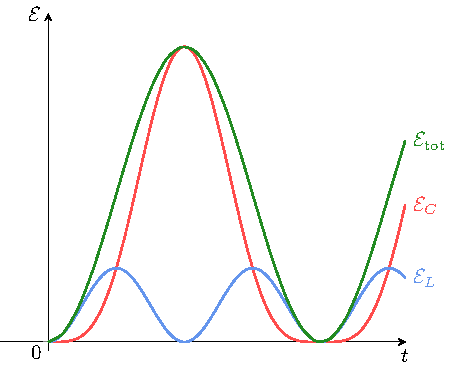
\includegraphics[width=\linewidth, draft=true]{carac-lc_montant-bilan}
			}{
				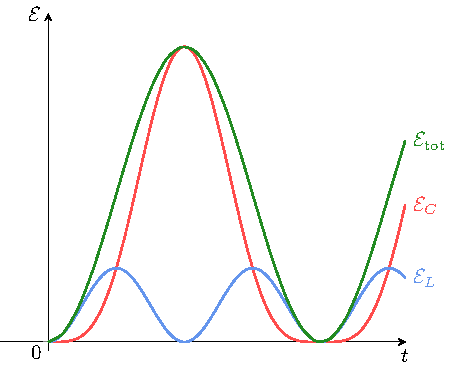
\includegraphics[width=\linewidth]{carac-lc_montant-bilan}
			}
			\captionof{figure}{}
		\end{center}
	\end{tcb}
\end{tcbraster}

\subsubsection{Intérêt oscillateur harmonique}

Le principal intérêt de l'observation régulière d'une oscillation est la mesure
du temps. Une excitation quelconque (comme un échelon) produit un phénomène se
reproduisant à intervalle régulier et fait alors apparaître un étalon
temporel. Ce principe est utilisé~:
\begin{itemize}
	\item dans les horloges mécaniques à balancier~: on exploite le mouvement
	      régulier du pendule~;
	\item dans les horloges à ressort~: la période est liée au rapport de
	      l'inertie et de la raideur du système~;
	\item dans les horloges électroniques~: un cristal de quartz dont la
	      fréquence d'oscillation est précisément connue (en général une puissance
	      de 2 en Hz)~;
	\item dans les horloges atomiques~: on utilise la régularité des
	      oscillations des ondes électromagnétiques absorbées par un atome.
	      L'actuelle définition de la seconde est basée sur le fonctionnement
	      d'une horloge atomique.
\end{itemize}

\section{Oscillateurs amortis}
\subsection{Introduction amorti}

\subsubsection{Évolutions en régime libre, exemple RLC}

\begin{minipage}{0.60\linewidth}
	En reprenant les résultats du LC libre, nous devrions en réalité observer que
	les oscillations dans le circuit s'atténuent. Soit le circuit RLC
	suivant\ftn{\url{https://tinyurl.com/ypbwcwfs}}, avec $L = \SI{43}{mH}$ et $C
		= \SI{20}{nF}$~:
\end{minipage}
\begin{minipage}{0.40\linewidth}
	\begin{center}
		\switch{
			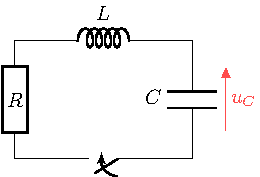
\includegraphics[width=.7\linewidth, draft=true]{rlc_descendant}
		}{
			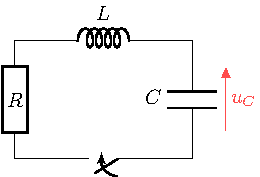
\includegraphics[width=.7\linewidth]{rlc_descendant}
		}
		\captionof{figure}{}
	\end{center}
\end{minipage}

\begin{itemize}
	\item Lorsque la \textbf{résistance est petite}~: on observe \textbf{plusieurs
		      oscillations}.
	      \bigbreak
	      On observe une série d'oscillations à la période $T \approx
		      \SI{184}{\micro s}$. On observe environ 25 oscillations lorsque $R
		      \approx \SI{60}{\ohm}$ (résistance interne du GBF + de la bobine), 9
	      oscillations lorsque $R \approx \SI{180}{\ohm}$, 5 oscillations lorsque
	      $R \approx \SI{500}{\ohm}$.
\end{itemize}
\begin{minipage}{0.45\linewidth}
	\begin{center}
		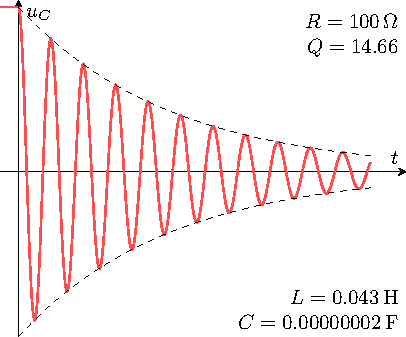
\includegraphics[width=\linewidth]{carac-rlc-15}
	\end{center}
\end{minipage}
\hfill
\begin{minipage}{0.45\linewidth}
	\begin{center}
		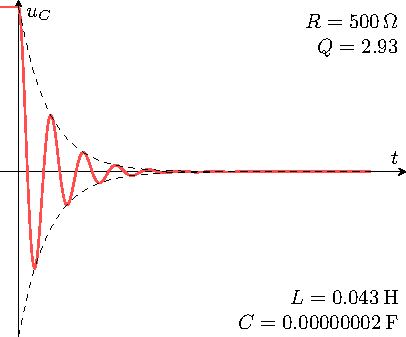
\includegraphics[width=\linewidth]{carac-rlc-3}
	\end{center}
\end{minipage}

\begin{itemize}
	\item Lorsque la \textbf{résistance est plus grande}~: les
	      \textbf{oscillations disparaissent}.
	      \bigbreak
	      Lorsque $R \approx \SI{2,9}{k\ohm}$, on
	      observe un régime transitoire dont la durée est d'environ $\SI{250}{\micro
			      s}$ (à 95\%). Lorsque $R \approx \SI{7.5}{k\ohm}$, on observe un régime
	      transitoire plus long, d'environ \SI{420}{\micro s}.
\end{itemize}
\begin{minipage}{0.45\linewidth}
	\begin{center}
		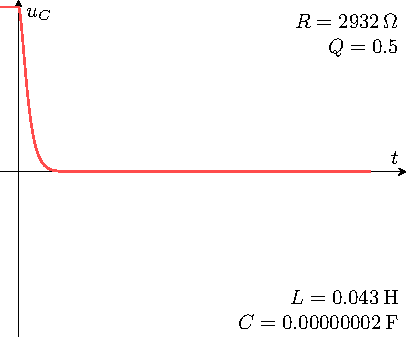
\includegraphics[width=\linewidth]{carac-rlc-05}
	\end{center}
\end{minipage}
\hfill
\begin{minipage}{0.45\linewidth}
	\begin{center}
		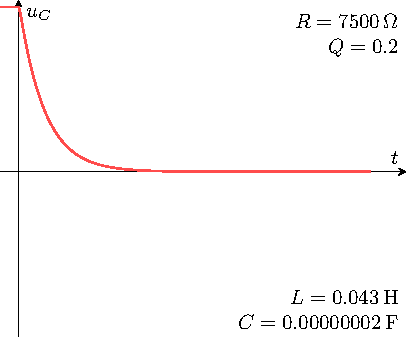
\includegraphics[width=\linewidth]{carac-rlc-02}
	\end{center}
\end{minipage}

\begin{tcb}(expe){Analyse}
	Lorsque l'on excite le système RLC, le système a deux principales réponses~:
	\begin{enumerate}
		\bitem{Système oscillant} pour $R < R_{c}$, de pseudo-période\ftn{On parle
			de \textit{pseudo}-période car le signal est diminué.} \textbf{supérieure à
			$T_0$}~;
		\bitem{Système non-oscillant} pour $R > R_c$~: le transitoire
		\textbf{augmente avec $R$}.
	\end{enumerate}
\end{tcb}

\subsubsection{Équation différentielle}

\begin{tcb}[label=prop:eqdiffoh](prop){Équation différentielle}
	Un oscillateur amorti à un degré de liberté est un système dont l'évolution
	temporelle est décrite par une grandeur $x(t)$ solution d'un équation
	différentielle du type~:
	\psw{
	\[
		\boxed{
		\dv[2]{x}{t} + \frac{\w_0}{Q} \dv{x}{t} + \w_0{}^2x =
		\w_0{}^2x_{\rm eq}
		}
	\]
	}
	Avec $x_{\rm eq}$ la position d'équilibre, $\w_0$ la pulsation
	\textbf{propre}, et $Q >0$ le \textbf{facteur de qualité}, sans dimension.
\end{tcb}
\begin{tcb}[label=impl:eqdiffamorti](impl)<lfnt>{Analyse de l'équation}
	Par lecture de cette équation, avec $Q$ sans dimension on retrouve que
	$\w_0$ s'exprime en \si{s^{-1}} car $\dv{x}{t}$ est de dimension
	$[x]\cdot\si{s^{-1}}$.
	\bigbreak
	De plus, on remarque que \textbf{plus $Q$ est élevé}, plus le terme
	d'ordre 1 est négligeable devant les autres, donc \textbf{plus on se
		rapproche de l'harmonique}.
	\bigbreak
	Le \textbf{facteur de qualité} traduit donc à quel
	point le système est \textbf{idéal}.
\end{tcb}

\subsubsection{Équation caractéristique et régimes de solutions}
\begin{tcb}[label=def:eqcarac, sidebyside](defi){Équation caractéristique}
	Pour résoudre une équation différentielle, on suppose une solution de la
	forme $x(t) = A\exp(rt)$ avec $r \in \Cb$. En injectant cette
	expression dans l'équation différentielle, on obtient l'\textbf{équation
		caractéristique}~:
	\psw{
		\begin{equation*}
			\boxed{r^2 + \frac{\w_0}{Q}r + \w_0{}^2 = 0}
		\end{equation*}
	}
	\tcblower
	C'est un trinôme du second degré, dont le discriminant $\Delta$ est
	\psw{
		\begin{equation*}
			\boxed{
				\Delta =
				\left( \frac{\w_0}{Q} \right)^2 - 4\w_0{}^2 =
				\frac{\w_0{}^{2}}{Q^{2}}\left( 1-4Q^{2} \right)
			}
		\end{equation*}
	}
\end{tcb}
\begin{tcb}[label=impl:eqcarac](impl){Régimes de solutions}
	Selon la valeur du discriminant, on aura différentes valeurs de $r$,
	doubles réelles, simple réelle ou doubles complexes. On a en effet
	\psw{
		\begin{gather*}
			\Delta > 0
			\Lra
			\frac{\cancel{\w_0{}^2}}{Q^2} - 4\cancel{\w_0{}^2} > 0
			\Lra
			Q^2 < \frac{1}{4}
			\Lra
			Q < \frac{1}{2}
		\end{gather*}
	}
	\vspace{-15pt}
	\begin{description}
		\item[$\mathbf{Q > 1/2}$] : régime \textbf{pseudo-périodique},
			racines complexes et oscillations décroissantes~;
		\item[$\mathbf{Q = 1/2}$] : régime \textbf{critique}, racine double
			réelle~;
		\item[$\mathbf{Q < 1/2}$] : régime \textbf{apériodique}, racines
			réelles et décroissance exponentielle sans oscillation.
	\end{description}
\end{tcb}

\begin{tcb}[label=nota:pm](nota){$\pm$ et $\mp$}
	Il est courant de noter les racines $r_\pm$ pour dénoter à la fois $r_+$ et
	$r_-$. Dans ce cas, l'expression de la racine contient le signe $\pm$, ce
	qui signifie que $r_+$ correspond à l'expression avec le $+$, et $r_-$
	correspond à l'expression avec le $-$.
	\smallbreak
	Si l'expression contient le signe $\mp$, c'est l'opposé~: $r_+$ correspond à
	l'expression avec $-$.
\end{tcb}

\begin{tcb}[label=prop:solureg, tabularx={Y|Y|Y}](ror){Solutions}
	\textbf{Pseudo-périodique} & \textbf{Critique} & \textbf{Apériodique}
	\\\hline
	$\D < 0 \Lra Q > 1/2$ & $\D = 0 \Lra Q = 1/2$ & $\D >
		0 \Lra Q < 1/2$
	\\\hline
	\begin{equation*}
		\boxed{r_\pm = - \frac{\w_0}{2Q} \pm \jj\W}
	\end{equation*}
	\begin{equation*}
		\boxed{\W = \frac{\w_0}{2Q}\sqrt{4Q^2 - 1}}
	\end{equation*}
	&
	\begin{equation*}
		\boxed{r = - \frac{\w_0}{2Q} = -\w_0}
	\end{equation*}
	&
	\begin{equation*}
		\boxed{r_\pm = \frac{\w_0}{2Q}\left(-1 \pm \sqrt{1 - 4Q^2}\right)}
	\end{equation*}
	\\\hline
	\begin{empheq}[box=\fbox]{gather*}
		x(t) = \underbrace{\exp \left(-\frac{\w_0}{2Q}t\right)}_{
			\text{partie décroissante}}\times\\
		\underbrace{\left[ A\cos(\Wt) + B\sin(\Wt) \right]}_{
			\text{partie oscillante}}
	\end{empheq}
	&
	\begin{equation*}
		\boxed{x(t) = (At + B)\exp(-\w_0t)}
	\end{equation*}
	&
	\begin{empheq}[box=\fbox]{gather*}
    x(t) = A\exp(r_+t) +\\
		\hspace{26pt} B\exp(r_-t)
	\end{empheq}
	\\
\end{tcb}

\subsection{Oscillateur amorti électrique~: circuit RLC série libre}
\subsubsection{Présentation}
\begin{minipage}[c]{.6\linewidth}
	\begin{itemize}
		\item Il est constitué de l'association en série d'une résistance, d'une
		      bobine et d'un condensateur idéaux.
		\item \textbf{On suppose le condensateur initialement chargé}~:
		      \fbox{$u_C(0^-) = E$ \underline{et} $i(0^-) = 0$} (condensateur chargé
		      $\equiv$ interrupteur ouvert).
		\item À $t=0$, on coupe le générateur.
	\end{itemize}
\end{minipage}
\hfill
\begin{minipage}[c]{.35\linewidth}
	~
	\begin{center}
		\switch{
			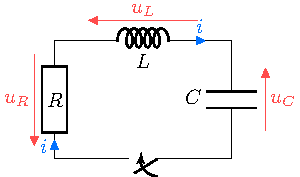
\includegraphics[width=.9\linewidth, draft=true]{rlc_descendant-intens}
		}{
			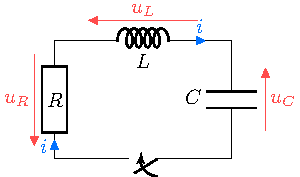
\includegraphics[width=.9\linewidth]{rlc_descendant-intens}
		}
		\captionof{figure}{}
	\end{center}
\end{minipage}

\subsubsection{Bilan énergétique}
\begin{tcb}[label=demo:rcenerg-charge](demo)<lfnt>{Bilan d'énergie}
	On fait un bilan de puissances~:
	\psw{
		\begin{DispWithArrows*}
			u_Ci + u_Li + u_Ri &= 0
			\Arrow{$i = C \dv{u_C}{t}$, $u_L = L \dv{i}{t}$ et $u_R = Ri$}
			\\\Lra
			u_C\times C \dv{u_C}{t} + L \dv{i}{t}\times i + Ri^2 &= 0
			\Arrow{$\Pc_J = Ri^{2}$ et $f \times f' = \left(\frac{1}{2}f^{2}\right)'$}
			\\\Lra
			\dv{}{t}
			\Big(
      \underbracket[1pt]{\frac{1}{2}C  u_C{}^2}_{\Ec_C} +
			\underbracket[1pt]{\frac{1}{2}Li^2}_{\Ec_L}
			\Big) &= -\Pc_J
		\end{DispWithArrows*}
	}
	\vspace{-15pt}
\end{tcb}
\begin{tcb}[label=prop:lcenerg-décharge](prop){Bilan d'énergie}
	L'énergie emmagasinée dans le circuit est progressivement dissipée par
	effet \textsc{Joule} dû à la résistance~:
	\psw{
		\[
			\boxed{\dv{\Ec}{t} = -\Pc_J}
		\]
	}
	avec $\Ec = \Ec_C + \Ec_L = \frac{1}{2}Cu_C{}^2 + \frac{1}{2}Li^2$.
\end{tcb}
\begin{tcb}[label=impo:amortissement, cnt, bld](impo){Résultat}
	On a donc bien une perte d'énergie à cause de la dissipation dans la
	résistance. Il y aura donc progressivement une perte de la tension
	de $u_C$, d'où l'amortissement.
\end{tcb}

\subsubsection{Équation différentielle du circuit}
\begin{tcb}[label=demo:eqdiffrc, sidebyside](demo)<lfnt>{Équation diff. RLC libre}
	Avec la loi des mailles,
	\psw{
		\begin{DispWithArrows*}[fleqn, mathindent=2pt]
			u_L + u_R = u_C &= 0
			\Arrow{$u_L = L \dv{i}{t}$\\et $u_R = Ri$}
			\\\Lra
			L \dv{i}{t} + Ri + u_C &= 0
			\Arrow{$i = C \dv{u_C}{t}$}
			\\\Lra
			LC \dv[2]{u_C}{t} + RC \dv{u_C}{t} + u_C                   &= 0
			\Arrow{forme\\canonique}
			\\
			\Lra \dv[2]{u_C}{t} + \frac{R}{L} \dv{u_C}{t} + \frac{1}{LC}u_C &= 0
		\end{DispWithArrows*}
	}
	\tcblower
	On détermine l'expression de $Q$ par identification~:
	\psw{
		\begin{DispWithArrows*}
			\frac{\w_0}{Q} &= \frac{R}{L}
			\Arrow{$\w_0 = \frac{1}{\sqrt{LC}}$}
			\\\Lra
			\frac{1}{Q \sqrt{LC}} &= \frac{R}{L}
			\Arrow{On isole $Q$}
			\\\Lra
			Q &= \frac{L}{R \sqrt{LC}}
			\Arrow{$L = \sqrt{L}^{2}$}
			\\\Lra
			\Aboxed{Q &= \frac{1}{R}\sqrt{\frac{L}{C}}}
		\end{DispWithArrows*}
	}
\end{tcb}
\begin{tcb}[label=prop:eqdiffrc, sidebyside,
		righthand ratio=.4](prop){Équation diff. RLC libre}
	L'équation différentielle de la tension $u_C(t)$ aux bornes d'un
	condensateur dans un circuit RLC en régime libre est
	\psw{
		\[
			\boxed{\dv[2]{u_C}{t} + \frac{\w_0}{Q} \dv{u_C}{t} + \w_0{}^2u_C = 0}
		\]
	}
	\begin{itemize}
		\item \fbox{$\w_0 = \frac{1}{\sqrt{LC}}$} la pulsation propre~;
		\item \fbox{$Q = \frac{1}{R} \sqrt{\frac{L}{C}}$} le facteur de
		      qualité.
	\end{itemize}
	\tcblower
	Les conditions initiales (continuité de $u_C$ aux bornes de $C$
	et de $i$ traversant $L$) sont
	\psw{
		\begin{empheq}[box=\fbox]{gather*}
			u_C(0^-) = u_C(0^+) = E\\
			i(0^-) = i(0^+) = 0
		\end{empheq}
	}
\end{tcb}

\subsubsection{Solutions}
\paragraph{Cas $\D < 0 \Lra Q > 1/2$~: régime pseudo-périodique}
~ \smallbreak
\begin{tcb}[label=demo:solupseudoper, breakable](demo)<lfnt>{Solution}
	On part de l'équation caractéristique~:
	\psw{
		\[
			r^{2} + \frac{\w_0}{Q}r + \w_0{}^{2} = 0
		\]
	}
	\vspace{-15pt}
	On a donc, avec $Q > 1/2$,
	\psw{
		\[
			\Delta = \frac{\w_0{}^{2}}{Q^{2}}\left( 1-4Q^{2} \right) < 0
		\]
	}
	\vspace{-15pt}
	Ainsi,
	\psw{
		\begin{DispWithArrows*}
			r_\pm & = \frac{-\frac{\w_0}{Q} \pm \jj\sqrt{-\D}}{2}
			\Arrow{On injecte $\Delta$}
			\\\Lra
			r_\pm &= -\frac{\w_0}{2Q} \pm
			\frac{\jj}{2} \sqrt{\frac{\w_0{}^{2}}{Q^{2}}\left( 4Q^{2}-1 \right)}
			\Arrow{On extrait $\frac{\w_0}{Q}$}
			\\\Lra
			r_\pm &= - \frac{\w_0}{2Q} \pm \jj \frac{\w_0}{2Q} \sqrt{4Q^{2}-1}
			\Arrow{On définit $\W$}
			\\\Lra
			r_\pm &= - \frac{\w_0}{2Q} \pm \jj\W
		\end{DispWithArrows*}
	}
	d'où la définition de $\W$~:
	\[
		\boxed{\W = \frac{\w_0}{2Q}\sqrt{4Q^{2}-1}}
	\]
	Ensuite, avec la forme générale de la solution on a
	\psw{
		\begin{equation*}
			u_C(t) = \exp \left(-\frac{\w_0}{2Q}t\right)
			\left[ A\cos(\Wt) + B\sin(\Wt) \right]
		\end{equation*}
	}
	\vspace{-15pt}
	\begin{itemize}
		\item On trouve $A$ avec la première condition initiale~:
		      \psw{
			      \begin{gather*}
				      u_C(0) = E = 1 \left[ A \cdot 1 + B \cdot 0 \right] = A
				      \quad \Ra \quad \boxed{A=E}
			      \end{gather*}
		      }
		      \vspace{-15pt}
		\item On trouve $B$ avec la seconde CI~:
		      \psw{
			      \begin{gather*}
				      \hspace*{-10pt}
				      \dv{u_C}{t} =
				      -\frac{\w_0}{2Q}\exp \left( -\frac{\w_0}{2Q}t \right)\times
				      \left[ A\cos(\Wt) + B\sin(\Wt) \right] +
				      \exp \left( -\frac{\w_0}{2Q}t \right)
				      \left[ -A\W\sin(\Wt) + B\W\cos(\Wt) \right]
				      \\\Ra
				      \dv{u_C}{t}\/(0) = - \frac{\w_0}{2Q}A + \W B = 0
				      \\\Lra
				      \boxed{B = \frac{\w_0}{2Q\W}E = \frac{E}{\sqrt{4Q^2-1}}}
			      \end{gather*}
		      }
	\end{itemize}
	% Ainsi, on trouve bien
	% \begin{empheq}[box=\fbox]{gather*}
	% 	u_C(t) = E\exp \left( -\frac{\w_0}{2Q}t \right)\times
	% 	\left[
	% 		\cos(\Wt) + \frac{1}{\sqrt{4Q^2 - 1}}\sin(\Wt)
	% 		\right]
	% \end{empheq}
\end{tcb}
\begin{tcb}[label=prop:solupseudoper, sidebyside](prop){Solution}
	Pour un facteur de qualité $Q > 1/2$, $u_C$ s'exprime par
	\psw{
		\begin{empheq}[box=\fbox]{gather*}
			u_C(t) = E\exp \left( -\frac{\w_0}{2Q}t \right)\times\\
			\left[
				\cos(\Wt) + \frac{1}{\sqrt{4Q^2 - 1}}\sin(\Wt)
				\right]
		\end{empheq}
	}
	avec
	\begin{equation*}
		\boxed{\W = \frac{\w_0}{2Q} \sqrt{4Q^2 - 1}}
	\end{equation*}
	La période des oscillations \textbf{diffère des oscillations harmoniques} $T_0
		= 2\pi/\w_0$ selon
	\psw{
		\begin{equation*}
			\boxed{
				T =
				\frac{2\pi}{\W} =
				\frac{2\pi}{\w_0} \frac{2Q}{\sqrt{4Q^{2} - 1}}
			}
		\end{equation*}
	}
	\tcblower
	Les oscillations se font entre les courbes
	\[y(t) = \pm E \exp \left( - \frac{\w_0}{2Q}t \right)\]
	\begin{center}
		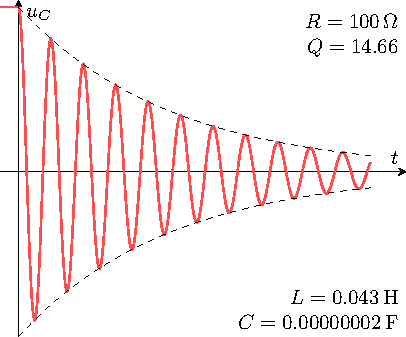
\includegraphics[width=\linewidth]{carac-rlc-15}
		\captionof{figure}{}
	\end{center}
\end{tcb}

\begin{tcb}[label=demo:transipseudo](demo)<lfnt>{Régime transitoire}
	L'amplitude varie selon $E\exp \DS \left( -\frac{\w_0}{2Q}t \right)$~; on
	définit donc $t_{95}$ tel que
	\psw{
		\begin{DispWithArrows*}
			\exp \left(-\frac{\w_0}{2Q}t_{95} \right) &= 0.05
			\Arrow{$\ln (~)$}
			\\\Lra
			- \frac{\w_0}{2Q}t_{95} &= \ln(0.05)
			\Arrow{$0.05 = 1/20$ et $\ln (a^{b}) = b \ln a$}
			\\\Lra
			\frac{\w_0}{2Q}t_{95} &= \ln(20)
			\Arrow{On isole}
			\\\Lra
			t_{95} &= 2\ln(20) \frac{Q}{\w_0}
		\end{DispWithArrows*}
	}
	Or $2\ln(20) \approx 2\pi$, d'où
\end{tcb}
\begin{tcb}[label=prop:transipseudo](prop)<lfnt>{Régime transitoire}
	Le temps de réponse à 95\% est atteint à partir de $t_{95}$ tel que
	\psw{
		\begin{equation*}
			\boxed{t_{95} \approx QT_0} \qav \boxed{T_0 = \frac{2\pi}{\w_0}}
		\end{equation*}
	}
	\vspace{-15pt}
\end{tcb}
\begin{tcb}[label=impo:pseudograndQ](impo){Résultat à grand $Q$}
	Avec ces résultats on remarque en effet que quand $Q \rightarrow \infty$, on
	a à la fois
	\begin{equation*}
		\boxed{\W \approx \w_0} \qdc \boxed{T \approx T_0}
	\end{equation*}
	Mais aussi
	\begin{equation*}
		\boxed{\dv[2]{u_C}{t} + \w_0{}^2u_C = 0} \qdc \boxed{u_C(t) = E\cos(\w_0t)}
	\end{equation*}
	On retrouve toutes les caractéristiques de la situation harmonique.
\end{tcb}

\begin{tcb}[breakable](rema){Visualisation dans l'espace des phases}
	Contrairement à la situation harmonique, le tracé de la solution dans
	l'espace $(u_C,i)$ n'est \textbf{pas symétrique par inversion du temps}~: la
	dissipation par effet \textsc{Joule} diminue l'énergie du système, et la
	\textbf{tension diminue progressivement}.
	\bigbreak
	On observera donc une \textbf{spirale décroissante} avec beaucoup
	d'oscillations quand les amortissements ne sont pas trop élevés, et de moins
	en moins quand $Q$ diminue ou que l'amortissement augmente.
	\tcblower
	\noindent
	\begin{minipage}{0.49\linewidth}
		\begin{center}
			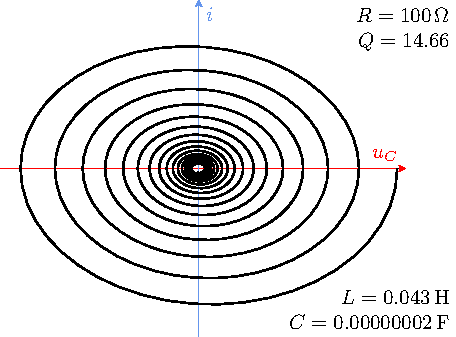
\includegraphics[width=.7\linewidth]{carac-rlc_xy-15}
			\captionof{figure}{Faible amortissement}
		\end{center}
	\end{minipage}
	\begin{minipage}{0.49\linewidth}
		\begin{center}
			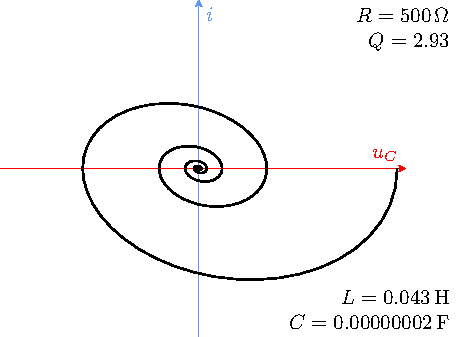
\includegraphics[width=.7\linewidth]{carac-rlc_xy-3}
			\captionof{figure}{Moyen amortissement}
		\end{center}
	\end{minipage}
\end{tcb}

\newpage
\paragraph{Cas $\D = 0 \Lra Q = 1/2$~: régime critique}
~\smallbreak
\vspace{-15pt}
\begin{tcb}[label=demo:solupseudoper](demo)<lfnt>{Solution}
	La seule racine de l'équation caractéristique est double, et vaut
	\psw{
		\[
			r = -\w_0
		\]
	}
	Ensuite, avec la forme générale de la solution on a
	\psw{
		\begin{equation*}
			u_C(t) = (At+B)\exp \left(-\w_0t\right)
		\end{equation*}
	}
	\vspace{-20pt}
	\begin{itemize}
		\item On trouve $B$ avec la première condition initiale~:
		      \psw{
			      \begin{gather*}
				      u_C(0) = E = (A\cdot0 + B)\cdot1 = B
				      \quad \Ra \quad \boxed{B=E}
			      \end{gather*}
		      }
		      \vspace{-15pt}
		\item On trouve $A$ avec la seconde CI~:
		      \psw{
			      \begin{gather*}
				      \dv{u_C}{t} = (A)\exp(-\w_0t) +
				      (At+E)(-\w_0)\exp(-\w_0t)
				      \\\Ra
				      \dv{u_C}{t}\/(0) = A -\w_0E = 0
				      \\\Lra
				      \boxed{A = \w_0E}
			      \end{gather*}
		      }
		      \vspace{-15pt}
	\end{itemize}
  \vspace{-30pt}
\end{tcb}
\begin{tcb}[label=prop:solupseudoper, sidebyside](prop){Solution}
	Pour un facteur de qualité $Q = 1/2$, $u_C$ s'exprime par
	\psw{
		\begin{empheq}[box=\fbox]{gather*}
			u_C(t) = E(\w_0t + 1) \exp(-\w_0t)
		\end{empheq}
	}
	et on n'observe \textbf{pas une oscillation}.
	\tcblower
	\begin{center}
		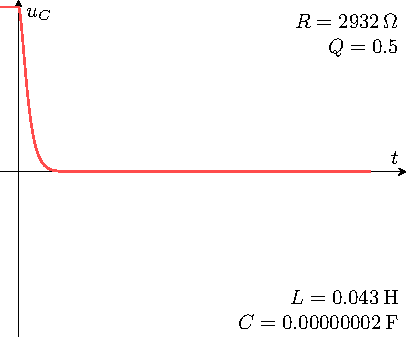
\includegraphics[width=\linewidth]{carac-rlc-05}
		\captionof{figure}{}
	\end{center}
\end{tcb}
\begin{tcb}[sidebyside](exem){Visualisation dans l'espace des phases}
	Au facteur de qualité critique, l'amortissement est suffisamment important
	pour empêcher $u_C$ de passer sous 0.
	\tcblower
	\begin{center}
		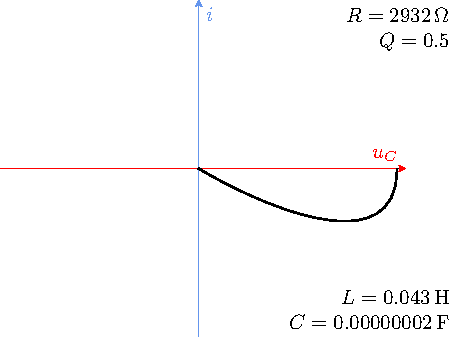
\includegraphics[width=.9\linewidth]{carac-rlc_xy-05}
		\captionof{figure}{}
	\end{center}
\end{tcb}
\begin{tcb}[label=demo:transicrit](demo)<lfnt>{Régime transitoire}
	En négligeant le terme linéaire en $t$ devant la décroissance
	exponentielle, on a
	\psw{
		\begin{gather*}
			\exp (-\w_0t_{95}) = \num{0.05} \Lra t_{95} =
			\frac{\ln(20)}{\w_0}
		\end{gather*}
	}
	\vspace{-15pt}
	Et avec $\ln(20) \approx \pi$ on a~:
\end{tcb}
\begin{tcb}[label=prop:transicrit](prop)<lfnt>{Régime transitoire}
	Le temps de réponse à 95\% est atteint à partir de $t_{95}$ tel que
	\psw{
		\begin{equation*}
			\boxed{t_{95} \approx \frac{T_0}{2}} \qav \boxed{T_0 = \frac{2\pi}{\w_0}}
		\end{equation*}
	}
	\vspace{-15pt}
\end{tcb}

\paragraph{Cas $\D > 0$~: régime apériodique}
~\smallbreak
\begin{tcb}[label=demo:solupseudoper, sidebyside](demo)<lfnt>{Solution}
	Les racines de l'équation caractéristique sont réelles, et on a
	\psw{
		\begin{gather*}
			r_\pm =
			\frac{- \frac{\w_0}{2Q}\pm\sqrt{\Delta}}{2}
			\\\Lra
			r_\pm = - \frac{\w_0}{2Q} \pm \frac{\w_0}{2Q} \sqrt{1 - 4Q^2}
			\\\Lra
			r_\pm = \frac{\w_0}{2Q} \left(-1 \pm \sqrt{1 - 4Q^2} \right)
		\end{gather*}
	}
	Ensuite, avec la forme générale de la solution on a
	\psw{
		\begin{equation*}
			u_C(t) = A \exp(r_+t) + B\exp(r_-t)
		\end{equation*}
	}
	\vspace{-15pt}
	\tcblower
	\begin{itemize}
		\item Avec la première CI~:
		      \psw{
			      \begin{gather*}
				      u_C(0) = E = A + B
			      \end{gather*}
		      }
		      \vspace{-15pt}
		\item Avec la seconde CI~:
		      \psw{
			      \begin{gather*}
				      \dv{u_C}{t}\/(0) = Ar_+ + Br_- = 0
				      \\\Lra
				      B = - \frac{Ar_+}{r_-}
			      \end{gather*}
		      }
		      \vspace{-15pt}
	\end{itemize}
	En combinant, on trouve
	\begin{equation*}
		\psw{
			\boxed{A = - \frac{Er_-}{r_+ - r_-}}
		}
		\qet
		\psw{
			\boxed{B = \frac{Er_+}{r_+ - r_-}
			}
		}
	\end{equation*}
	D'où le résultat~:
\end{tcb}
\begin{tcb}[label=prop:solupseudoper, sidebyside](prop){Solution}
	Pour un facteur de qualité $Q < 1/2$, $u_C$ s'exprime par
	\psw{
		\[
			\boxed{
				u_C(t) =
				\frac{E}{r_+-r_-} \left( r_+\exp(r_-t) - r_-\exp(r_+t) \right)
			}
		\]
	}
	et on n'observe \textbf{pas une oscillation}. Le régime transitoire est
	\textit{plus long} que pour $Q = 1/2$.
	\tcblower
	\begin{center}
		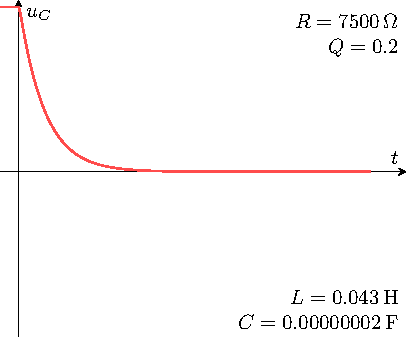
\includegraphics[width=\linewidth]{carac-rlc-02}
		\captionof{figure}{}
	\end{center}
\end{tcb}

\begin{tcb}[sidebyside](exem){Visualisation dans l'espace des phases}
	Pendant le régime apériodique, l'amortissement est suffisamment important pour
	non seulement empêcher $u_C$ d'osciller, mais également pour \textbf{ralentir
		sa diminution }vers $0$. Son trajet se fait donc à une vitesse plus faible,
	c'est-à-dire $\dv{u_C}{t}$ plus petit donc $i$ plus petit.
	\tcblower
	\begin{center}
		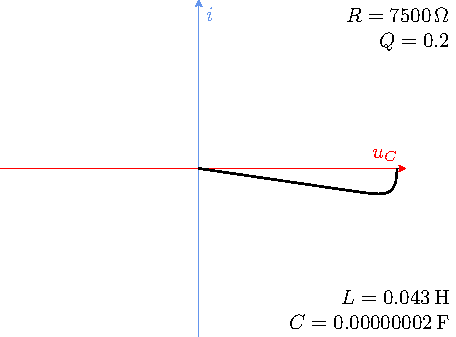
\includegraphics[width=\linewidth]{carac-rlc_xy-02}
		\captionof{figure}{}
	\end{center}
\end{tcb}
\begin{tcb}[label=demo:transiaper](demo)<lfnt>{Régime transitoire}
	La décroissance sera guidée par l'exponentielle la «~\textbf{moins
		décroissante}~». On cherche donc à savoir laquelle, on compare donc $r_-$ et
	$r_+$.
	\smallbreak
	On remarque d'abord que les deux racines sont négatives (d'où la
	décroissance exponentielle). En effet,
	\vspace{-15pt}
	\psw{
		\begin{align*}
			r_+ < 0
			 & \Lra
			\underbrace{\cancel{-\frac{\w_0}{2Q}}}_{\w_0 \text{ et } Q > 0}
			\left( 1 - \sqrt{1-4Q^2}
			\right) \underbrace{\cancel{<}}_{>} 0
			\\&\Lra
			1 - \sqrt{1 - 4Q^2} > 0
			\\&\Lra
			\sqrt{1-4Q^2}^{2} < 1^{2}
			\\&\Lra
			4Q^2 > 0
		\end{align*}
	}
	\vspace{-15pt}
	ce qui est vrai. Or,
	\psw{
		\begin{DispWithArrows*}[]
			r_- &< r_+
			\Arrow{$\abs{~}$}
			\\\Lra
			\abs{r_-} &> \abs{r_+}
			\Arrow{$(~)^{-1}$}
			\\\Lra
			\abs{\frac{1}{r_-}} &< \abs{\frac{1}{r_+}}
			\Arrow{$\tau = \abs{1/r}$}
			\\\Lra
			\tau_- &< \tau_+
		\end{DispWithArrows*}
	}
	On estime alors la durée du régime transitoire à
	\fbox{$\ln(20)/\abs{r_+}$}.
	\bigbreak
	Pour $Q \ll 1$, on utilise \fbox{$\sqrt{1+x} \underset{x\ll1}{\approx}
			1+x/2$} pour simplifier $r_+$~:
	\psw{
		\begin{gather*}
			r_+ =
			-\frac{\w_0}{2Q} \left( 1 - \sqrt{1-4Q^{2}} \right)
			\\\Ra
			r_+ \underset{Q\ll1}{\approx}
			- \frac{\w_0}{2Q} \left( 1 - \left(1 - \frac{4Q^2}{2}\right) \right)
			\\\Lra
			r_+ \underset{Q\ll1}{\approx} -Q\w_0
		\end{gather*}
	}
	Avec $\ln(20) \approx \pi$, on a finalement
	\psw{
		\begin{equation*}
			\boxed{t_{95} \approx \frac{\pi}{Q\w_0}} \qso \boxed{t_{95} \approx
				\frac{T_0}{2Q}}
		\end{equation*}
	}
	\vspace{-15pt}
\end{tcb}

\begin{tcb}[label=prop:transiaper](prop)<lfnt>{Régime transitoire}
	Le temps de réponse à 95\% est atteint à partir de $t_{95}$ tel que
	\psw{
		\begin{equation*}
			\boxed{
				t_{95} \approx \frac{T_0}{2Q}} \qav \boxed{T_0 =
				\frac{2\pi}{\w_0}
			}
		\end{equation*}
	}
\end{tcb}
\begin{tcb}[label=impo:aperpetitQ](impo){Résultat à faible $Q$}
	Quand $Q \longrightarrow 0$, on peut négliger le terme d'ordre 2 dans
	l'équation différentielle, soit
	\begin{gather*}
		\frac{\cancel{\w_0}}{Q}\dv{u_C}{t} +
		\w_0{}^{\cancel{2}}u_C = R \sqrt{\frac{C}{L}} \dv{u_C}{t} +
		\frac{1}{\sqrt{LC}}u_C \\
		=
		\dv{u_C}{t} + \frac{1}{R}
		\sqrt{\frac{\bcancel{L}}{\bcancel{L}C^2}} u_C
		=
		\boxed{ \dv{u_C}{t} +
			\frac{1}{RC} u_C}
	\end{gather*}
	d'où la décroissance exponentielle. D'autre part, les valeurs de $r_\pm$
	tendent vers la même valeur $r = - \frac{\w_0}{2Q}$~: en supposant la solution
	comme la somme des deux racines, on aurait une décroissance en
	\begin{gather*}
		r = -\frac{\w_0}{Q} = - \frac{1}{\sqrt{LC}}R
		\sqrt{\frac{C}{L}}
		\Lra
		r = -R \sqrt{\frac{\cancel{C}}{L^2\cancel{C}}}
	\end{gather*}
	soit une décroissance exponentielle avec un temps
	caractéristique $\tau = \frac{L}{R}$.
\end{tcb}

\vspace{-15pt}
\subsection{Exemple amorti mécanique~: ressort + frottements fluides}

\subsubsection{Présentation}
\begin{tcb}[label=def:ressortlibre, sidebyside](defi){Situation
			initiale et bilan des forces}
	\begin{itemize}[label=$\diamond$, leftmargin=10pt]
		\bitem{Système~:} \{point M\} de masse $m$, accroché à un \textbf{ressort
			idéal avec frottements}
		\bitem{Référentiel~:} $\Rc\ind{sol}(O',x,y,t)$ supposé galiléen
		\bitem{Repère~:} $(\Or', \ux, \uy)$ (voir schéma)
		\bitem{Repérage~:}
		\vspace{-15pt}
		\begin{center}
			\hspace*{-10pt}
			\fbox{Soit $x (t) = \ell(t) - \ell_0$ la position de la masse}
		\end{center}
		\[
			\vv{\rm O'M} = x(t)\ux~; \vf = \xp(t)\ux~; \af = \xpp(t)\ux.
		\]
		\bitem{Position initiale~:} ${\rm O'M}(0) = x_0 >0$
		\bitem{Vitesse initiale~:} $\vf(0) = \of$
	\end{itemize}
	\tcblower
	\begin{center}
		\switch{
			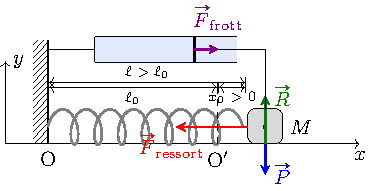
\includegraphics[width=\linewidth, draft=true]{ressort_amorti}
		}{
			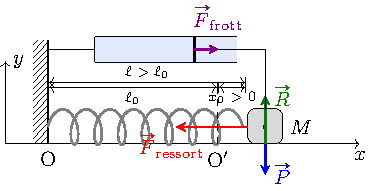
\includegraphics[width=\linewidth]{ressort_amorti}
		}
		\captionof{figure}{}
	\end{center}
	\begin{itemize}[label=$\diamond$, leftmargin=10pt]
		\bitem{Bilan des forces~:}
		\psw{
			\[
				\begin{array}{ll}
					\textbf{Poids}               & \Pf = m\gf = -mg \uy         \\
					\textbf{Réaction normale}    & \Rf = R\uy                   \\
					\textbf{Force de rappel}     & \Ff = -kx (t)\ux             \\
					\textbf{Force de frottement} & \Ff_{\rm frott} = -\alpha\vf
				\end{array}
			\]
		}
	\end{itemize}
\end{tcb}

\subsubsection{Équation différentielle}

\begin{tcbraster}[raster columns=2, raster equal height=rows]
	\begin{tcb}[label=prop:eqdiffreslibre](prop){Équation et solution}
		La position $x$ de la masse et la longueur $\ell$ du ressort sont régies
		par~:

		\begin{empheq}[box=\fbox]{gather*}
			\dv[2]{x}{t} + \frac{\w_0}{Q} \dv{x}{t} + \w_0{}^2x = 0\\
			\Lra \dv[2]{\ell}{t} +
			\frac{\w_0}{Q} \dv{\ell}{t} + \w_0{}^2\ell = \w_0{}^2\ell_0
		\end{empheq}
		\begin{itemize}
			\item \fbox{$\w_0 = \frac{k}{m}$} la pulsation propre~;
			\item \fbox{$Q = \frac{\sqrt{km}}{\alpha}$} le facteur de qualité.
		\end{itemize}
		$\ell_0$ \textbf{reste} donc la longueur d'équilibre du système.
	\end{tcb}
	\begin{tcb}[label=demo:solreslibre](demo)'r'{Équation différentielle}
		Avec le PFD~:
		\psw{
			\begin{gather*}
				m\af = \Pf + \vv{R} + \Ff\\
				\Lra m\left(
				\begin{array}{c}
						\dv[2]{x}{t} \\
						0
					\end{array}
				\right)
				=
				\left(
				\begin{array}{c}
						-kx -\alpha v \\
						-mg + R
					\end{array}
				\right)
			\end{gather*}
		}
		Sur l'axe $\ux$ on trouve donc
		\psw{
			\[
				m \dv[2]{x}{t} + \alpha \dv{x}{t} + kx = 0
			\]
		}
		\vspace{-15pt}
	\end{tcb}
\end{tcbraster}

\begin{tcb}[sidebyside, righthand ratio=.4](impo){Analogie RLC-ressort amorti}
	Ici aussi, les deux systèmes sont \textbf{régis par la même équation
		différentielle}. On observe une \textbf{oscillation amortie} du ressort
	autour d'une position d'équilibre, ici $x=0 \Lra \ell = \ell_0$.
	\bigbreak
	Ici, c'est le coefficient de frottements $\alpha$ qui dissipe~: on l'associe
	à $R$.
	\smallbreak
	\tcblower
	\captionof{table}{Correspondances}
	\centering
	\begin{tabular}{c@{$\longleftrightarrow$}c}
		\toprule
		Méca                       & Élec
		\\
		\midrule
		\psw{$x$}                  & \psw{$q$}
		\\
		\psw{$v$}                  & \psw{$i$}
		\\
		\psw{$m$}                  & \psw{$L$}
		\\
		\psw{$k$}                  & \psw{$C^{-1}$}
		\\
		\psw{$\sqrt{\frac{k}{m}}$} & \psw{$\frac{1}{\sqrt{LC}}$}
		\\
		\psw{$\alpha$}             & \psw{$R$}
		\\
		\bottomrule
	\end{tabular}
\end{tcb}

\subsubsection{Bilan énergétique}

\begin{tcbraster}[raster columns=2, raster equal height=rows]
	\begin{tcb}[label=prop:emecacons](prop){Conservation énergie}
		Dans le système masse-ressort horizontal avec frottements fluides,
		l'énergie mécanique diminue progressivement proportionellement au
		coefficient de friction $\alpha$~:
		\psw{
			\begin{equation*}
				\boxed{\dv{\Ec_{m}}{t} = -\alpha v^2}
			\end{equation*}
		}
	\end{tcb}
	\begin{tcb}[label=demo:emecacons](demo)'r'{Conservation énergie}
		À partir du PFD $\times v$~:
		\psw{
			\begin{gather*}
				m \dv[2]{x}{t} \dv{x}{t} + \alpha \dv{x}{t} \dv{x}{t} + kx \dv{x}{t} = 0\\
				\Lra \dv{}{t} \left( \frac{1}{2}m \left( \dv{x}{t} \right)^2 +
				\frac{1}{2}kx^2 \right) = - \alpha v^2
			\end{gather*}
		}
		On a bien $\Ec_m = \Ec_C + \Ec_{p, \rm el}$ qui diminue.
	\end{tcb}
\end{tcbraster}

\subsubsection{Solutions}
\begin{center}
	\begin{tcb}[label=prop:ressortsolu](prop){Solutions}
		\begin{center}
			\textbf{On a les mêmes solutions en changeant $u_C$ par $x$ et $E$
				par $x_0$}
		\end{center}
	\end{tcb}
\end{center}

\subsubsection{Résumé oscillateurs amortis}
\begin{tcb}[label=ror:resumeamorti, tabularx={Y|Y|Y}](ror){Résumé -- à ne pas
  connaître par cœur~!}
	\textbf{Pseudo-périodique} & \textbf{Critique} & \textbf{Apériodique}
	\\\hline
	$\D < 0 \Lra Q > 1/2$ & $\D = 0 \Lra Q = 1/2$ & $\D >
		0 \Lra Q < 1/2$
	\\\hline
	\begin{equation*}
		\boxed{r_\pm = - \frac{\w_0}{2Q} \pm \jj\W}
	\end{equation*}
	\begin{equation*}
		\boxed{\W = \frac{\w_0}{2Q}\sqrt{4Q^{2} - 1}}
	\end{equation*}
	&
	\begin{equation*}
		\boxed{r = - \frac{\w_0}{2Q} = -\w_0}
	\end{equation*}
	&
	\begin{equation*}
		\boxed{r_\pm = \frac{\w_0}{2Q}\left(-1 \pm \sqrt{1 - 4Q^2}\right)}
	\end{equation*}
	\\\hline
	\begin{empheq}[box=\fbox]{gather*}
		u_C(t) = E\exp \left( -\frac{\w_0}{2Q}t \right)\times\\
		\hspace*{-3pt}
		\left[
			\cos(\Wt) + \frac{1}{\sqrt{4Q^2 - 1}}\sin(\Wt)
			\right]
	\end{empheq}
	&
	\begin{empheq}[box=\fbox]{gather*}
		u_C(t) = E(\w_0t + 1) \exp(-\w_0t)
	\end{empheq}
	&
	\begin{empheq}[box=\fbox]{gather*}
    u_C(t) = \frac{E}{r_+-r_-}\times\\
    \big(r_+\exp(r_-t) - r_-\exp(r_+t) \big)
	\end{empheq}
	\\\hline
	$t_{95} \approx QT_0$ &
	\[t_{95} \approx \frac{T_0}{2}\] &
	\[t_{95} \approx \frac{T_0}{2Q}\]
	\\\hline
	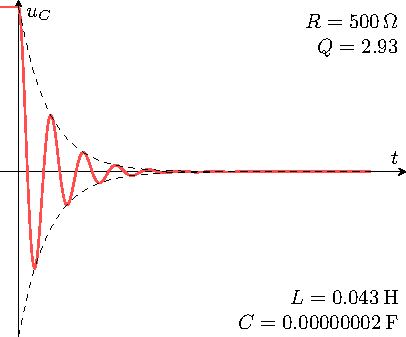
\includegraphics[width=\linewidth]{carac-rlc-3} &
	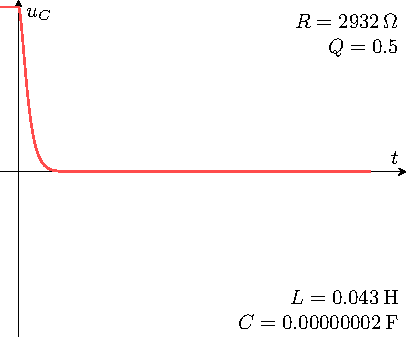
\includegraphics[width=\linewidth]{carac-rlc-05} &
	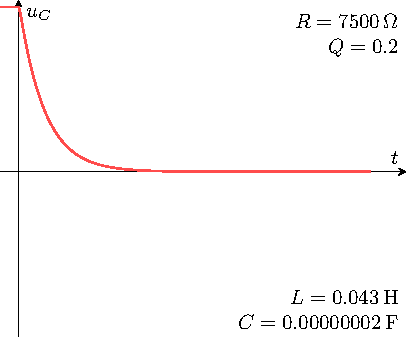
\includegraphics[width=\linewidth]{carac-rlc-02}
	\\\hline
	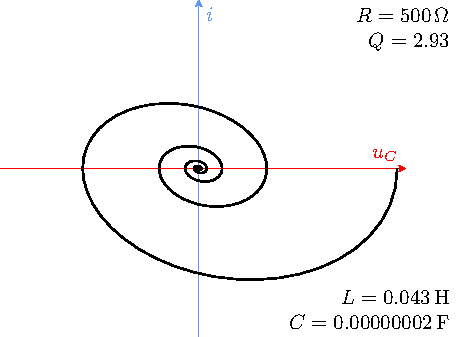
\includegraphics[width=\linewidth]{carac-rlc_xy-3} &
	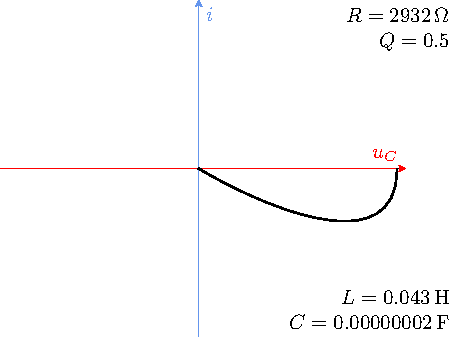
\includegraphics[width=\linewidth]{carac-rlc_xy-05} &
	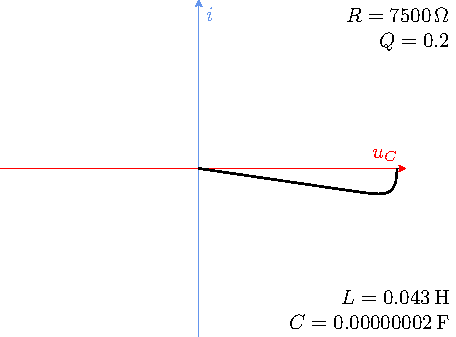
\includegraphics[width=\linewidth]{carac-rlc_xy-02}
	\\\hline
\end{tcb}

\end{document}
